\documentclass{article}
\usepackage{amsfonts, amsmath, amssymb, amsthm} % Math notations imported
\usepackage{enumitem}
\usepackage[margin=1in]{geometry}
\usepackage{graphicx}
\graphicspath{{./images/}} % Path to images


\newtheorem{thm}{Theorem}
\newtheorem{prop}[thm]{Proposition}
\newtheorem{cor}[thm]{Corollary}

% title information
\title{Math 154 HW6}
\author{Neo Lee}
\date{05/24/2023}

% main content
\begin{document} 

% placing title information; comment out if using fancyhdr
\maketitle 

\textbf{Problem 1.}
Use the greedy algorithm with vertex ordering A, B, C, D, E, F to color the graph below. 
Does a coloring with fewer colors exist? Why or why not?
\begin{proof}[Solution] \indent 
    \begin{figure}[htb!]
        \centering
        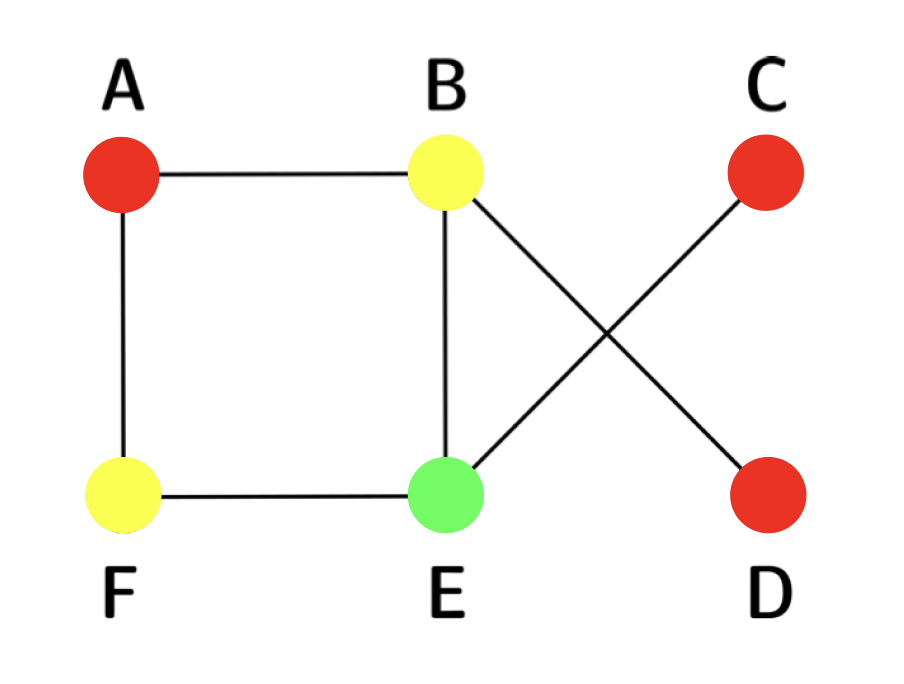
\includegraphics[scale=0.5]{coloring.png}
        \caption{Coloring of the graph.}
    \end{figure}

    The greedy algorithm with vertex ordering A, B, C, D, E, F colors the graph with 3 colors.
    However, a coloring with fewer colors does exist.
    Notice that there is no odd cycle in the graph, so the graph is in fact bipartite.
    Hence, we can color the graph with 2 colors.
\end{proof}
\bigbreak

\textbf{Problem 2.}
Let $\omega(G)$ be the maximum number of vertices in a complete subgraph of a graph $G$.
\begin{enumerate}[label=(\alph*)]
    \item 
    \begin{prop}
        For every graph $G$, $\chi(G) \ge \omega(G)$.
    \end{prop}
    \begin{proof}
        Let $G'$ be the complete subgraph of $G$ with $\omega(G)$ vertices.
        Then considering $G'$ only, we know that $\chi(G') = \omega(G)$ by Brooks' theorem.
        Since $G'$ is a subgraph of $G$, we know that $\chi(G') \le \chi(G)$.
        Hence, $\chi(G) \ge \omega(G)$.
    \end{proof}

    \item
    \begin{prop}
        For every graph $G$, $\chi(G) \ge \frac{|V(G)|}{\alpha(G)}$.
    \end{prop}
    \begin{proof}
        By definition, $\chi(G)$ is the minimum number of independent sets that partition $V(G)$. 
        Let's denote $\{A_1, \dots, A_{\chi(G)}\}$ to be the partition, in which $|A_k| \le \alpha(G)\; \forall k \in [1,\chi(G)]$.
        Hence, $\alpha(G)\chi(G) \ge \sum_{k=1}^{\chi(G)}A_k = |V(G)| \Leftrightarrow \chi(G) \ge \frac{|V(G)|}{\alpha(G)}$.
    \end{proof}
\end{enumerate}
\bigbreak

\textbf{Problem 3.}
Suppose we have a computer program with 6 variables, as summarized in this table. 
\begin{displaymath}
    \begin{array}{|c|c|}
        \hline
        \text{Variable} & \text{Steps used} \\
        \hline
        a & 1-2 \\
        b & 1-5 \\
        c & 6-8 \\
        d & 3-10 \\ 
        e & 4-7 \\
        f & 9-10 \\
        \hline
    \end{array}
\end{displaymath}
(Here, a and b can’t be stored in the same register, because both are used in Steps 1-2, but for example, a and c could be, since they’re not used simultaneously.)

If we want to store each variable in a register, what is the minimum number of registers needed to run this program? (Note: you should convert this into a graph theory problem before solving it!)
\begin{proof}[Solution]
    The question can be framed as a graph theory problem concerned with the following graph $G$.
    \begin{figure}[htb!]
        \centering
        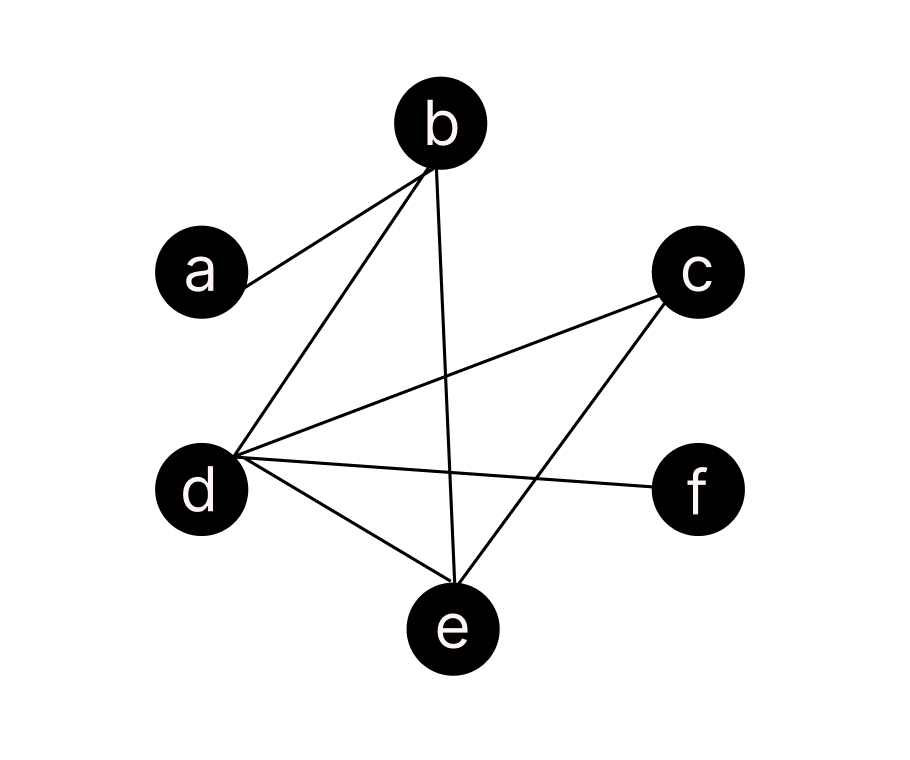
\includegraphics[scale=0.3]{hw6-3.png}
        \caption{Graph $G$}
    \end{figure}

    The minimum number of registers needed to run this program is the chromatic number of $G$.
    Notice there is a triangle in $G$, so $\chi(G) \ge 3$.
    Now, notice that $G$ is \emph{2-degenerate}. 
    Then, we can perform greedy coloring on $G$ with the following ordering: $a, f, b, c, d, e$, which would take 3 colors.
    Therefore, $\chi(G) \le 3$.
    Hence, the minimum number of registers needed to run this program is 3.
\end{proof}

\bigbreak

\textbf{Problem 4.}
\begin{prop}
    If m is the length of the longest path in a graph G, $\chi(G) \le m + 1.$
\end{prop}
\begin{proof}
    Let $v_1$ be the vertex at the end of the longest path in $G$.
    Then, $v_1$ has at most $m$ neighbors, otherwise contradiction and there exists a longer path by appending the extra neighbor to the path.

    Now, we remove $v_1$ to get $G'$. Notice the longest path length in $G'$ is at most $m$.
    Then, the end point, let $v_2$, of the longest path in $G'$ has at most $m$ neighbors.
    This is always true when we remove the end point of the longest path in $G$ iteratively.

    Therefore, we can form an arrangement of the vertices by iteratively removing the end point of the current longest path in the subgraph.
    Denote the arrangement as $(v_1, v_2, v_3, \dots, v_n)$. Notice for each $v_k$, $k \in [1, n]$, $v_k$ has at most $m$ neighbors in the subgraph induced by $\{v_k, v_{k+1}, \dots, v_n\}$.
    Then, we can perform greedy coloring starting from $v_n$, which would produce a coloring with at most $m+1$ colors.

    Notice, there is a caveat that when we remove $v_k$ from the subgraph, it may break into multiple components.
    However, this does not affect the proof, since we can just color the components separately, and as a matter of fact, it would make the coloring even easier.
\end{proof}

\end{document}